\scanpage{100}
% archive foliation: 101
$(\text{iv})\Longrightarrow(\text{ii bis})$

Soit $S_j$ la condition $\boxed{\operatorname{Ker}f^j\subset\operatorname{Im}f^{n-j}}$

Prouvons que si $1\leq j\leq n-1$, alors \uline{$S_j\Longrightarrow S_{j-1}$}

\deleted{Soit $\unsure{x\in fA}$} prouvons $\operatorname{Ker}f^{j-1}\subset\operatorname{Im}f^{n-j+1}$

$\operatorname{Ker}f^{j-1}\subset\operatorname{Ker}f^j\subset\operatorname{Im}f^{n-j}\subset\operatorname{Im}f$ d'où
\[
\operatorname{Ker}f^{j-1}=f^{\deleted{\unsure{n-j}}}(\operatorname{Ker}f^{j\deleted{\unsure{+n-j-1}}})
\deleted{\unsure{\subset f^{n-j}(\operatorname{Ker}f^{n-1})=f(\underbrace{f^{n-j}(\operatorname{Ker}f^{n-1})}_{\subset f^{n-j}(A)})}}
\inserted{\subset f(\operatorname{Im}f^{n-j})=\operatorname{Im}f^{n-j+1}}
\]
\diagram{\begin{tikzcd}
\operatorname{Ker}f^{j-1}&&\\
x\arrow[u,phantom,"\rotatebox{90}{$\in$}" description]\arrow[r,leftrightarrow]&{}&
\end{tikzcd}}
\diagram{\begin{tikzcd}[column sep=large]
\deleted{x=f^{n-j}(y)}\arrow[dd,bend right,no head]\arrow[ddr,no head]&\deleted{f^{n-1}y=0}\\
&f^j(f^{n-j-1}y)=0\\
&f^{n-1-j}y=f^{n-j}z
\end{tikzcd}}
OK

Donc on trouve de proche en proche
\[
S_j\Longrightarrow S_1\quad\text{i.e.}\quad\operatorname{Ker}f\subset\operatorname{Im}f^{n-1}
\]
donc $f$ induit un hom \uline{injectif} donc \uline{bijectif}
\[
A/f^{n-1}A\xrightarrow{f}fA.
\]
Comme sur les \unsure{gr. dérivés} associés c'est surjectif, c'est aussi \uline{bijectif} sur les \unsure{gr. dérivés} associés, c'est exactement (i).

\figure{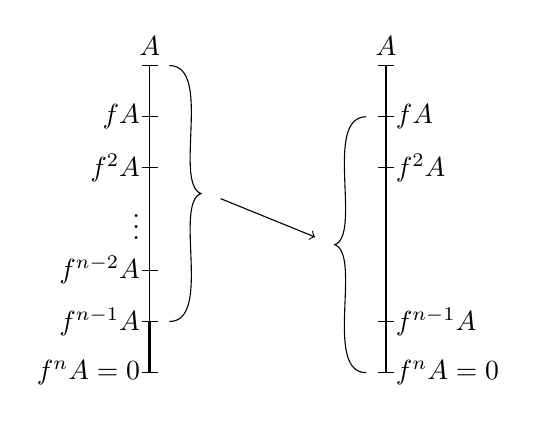
\begin{tikzpicture}[x=1cm,y=.65cm]
\draw (0,0)--(0,6);\draw[very thick] (0,0)--(0,1);
\draw (3,0)--(3,6);
\foreach \y in {0,1,2,4,5,6}{\draw (-.1,\y)--(.1,\y);}
\foreach \y in {0,1,4,5,6}{\draw (2.9,\y)--(3.1,\y);}
\node[above] at (0,6){$A$};\node[left] at (0,5){$fA$};\node[left] at (0,4){$f^2A$};\node[left] at (0,3){$\vdots$};\node[left] at (0,2){$f^{n-2}A$};\node[left] at (0,1){$f^{n-1}A$};\node[left] at (0,0){$f^nA=0$};
\node[above] at (3,6){$A$};\node[right] at (3,5){$fA$};\node[right] at (3,4){$f^2A$};\node[right] at (3,1){$f^{n-1}A$};\node[right] at (3,0){$f^nA=0$};
\draw (.25,6) .. controls (.8,6) and (.3,3.7) .. (.65,3.5) .. controls (.3,3.3) and (.8,1) .. (.25,1);
\draw (2.75,5) .. controls (2.2,5) and (2.7,2.7) .. (2.35,2.5) .. controls (2.7,2.3) and (2.2,0) .. (2.75,0);
\draw[->] (.9,3.4)--(2.1,2.65);
\end{tikzpicture}}

\figure{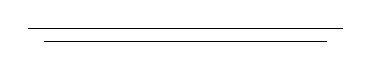
\begin{tikzpicture}\draw (0,0)--(4,0);\draw (.2,-.17)--(3.8,-.17);\end{tikzpicture}}
\margin{\uline{Terminologie}: Obj $A$ de \deleted{\unsure{tors.}}, de \deleted{\unsure{longueur}} \inserted{\unsure{rg}} $n$}

Supposons que l'on ait sur $\mathcal C$ une fonction \unsure{à} valeurs entières, additif pour les extensions, et qui est nulle ssi l'argument est nul. Alors ces conditions impliquent que
$\operatorname{rg}(A)=n\operatorname{rg}(A/fA)$.

\deleted{Un hom} Si $B$ est \deleted{\unsure{comme $A$}}, \deleted{\unsure{muni}} de $g$, \deleted{$B$} satisfait les conditions analogues pour $(g,n)$,
\deleted{\unsure{donc}} et si $u:A-B$ est un hom compatible aux $f,g$, \deleted{\unsure{et}} si on suppose que $\operatorname{rg}(A/fA)=\operatorname{rg}(B/gB)$, alors

Conditions équivalentes

(i) $u$ est \unsure{monomorphisme}

\unsure{(i bis)} $u$ \unsure{un épimorphisme}

\unsure{(i ter)} $u$ \unsure{un isomorphisme}

\diagram{\begin{array}{lll}
\unsure{\text{(ii)}}&\operatorname{gr}^0(u)\text{ est un}&\left\{\begin{array}{l}\unsure{\text{monomorphisme}}\\\text{épimorphisme}\\\text{isomorphisme}\end{array}\right.\\
\unsure{\text{(ii bis)}}&\unsure{\operatorname{gr}^0(u)}&\unsure{\Longrightarrow}\\
\unsure{\text{(iii bis)}}&\unsure{\operatorname{gr}^i(u)}&\unsure{\Longrightarrow}
\end{array}}
\margin{\deleted{$\unsure{R_D}$} \unsure{déf. rg d'obj de BT}$=\operatorname{rg}(A/fA)$}
\margin{$\unsure{\frac{p\times\ell}{e}x=\left[\frac{p\times\ell}{e}(x)\right]}$}
\margin{\unsure{$\varphi$|$\ell$}\quad\unsure{$\frac{\ell}{e}\longleftarrow\frac{R_D}{e}x$}}
